\graphicspath{{chapters/images/02/}}

\Chapter{NGS principles}
NGS stands for Next Generation Sequencing, and it represents the method of sequencing most used nowadays.

\section{History of Sequencing}
The first method ever used to sequence DNA was designed by Frederick Sanger. The Sanger manual sequencing system consists in the process described in figure \ref{•}, also named as "primer extension".



Some single-filament DNA molecules, which are the templates to be sequenced, were charged over an electrophoretical gel made in polyacrilamide.



as the time passes, the cost of sequencing DNA is diminishing. After the Human genome project, several other animals and plants' genomes were sequenced.

several diverse approaches are possible to sequence DNA.
\begin{itemize}
	\item \textbf{Chemical degradation of DNA} which includes the method of Maxam and Gilbert
	\item \textbf{Sequencing by synthesis (“SBS”)} which is the most common approach and the first to be developed. Illumina, Pacific Bioscences, Ion Torren...
	\item \textbf{Ligation-based}: sequencing using short probes that hybridize to the template % SOLiD, Complete Genomics
	\\textbf{Other:} Nanopore
\end{itemize}

\begin{figure}[h]
\caption{The sequencing machines available today}
\centering
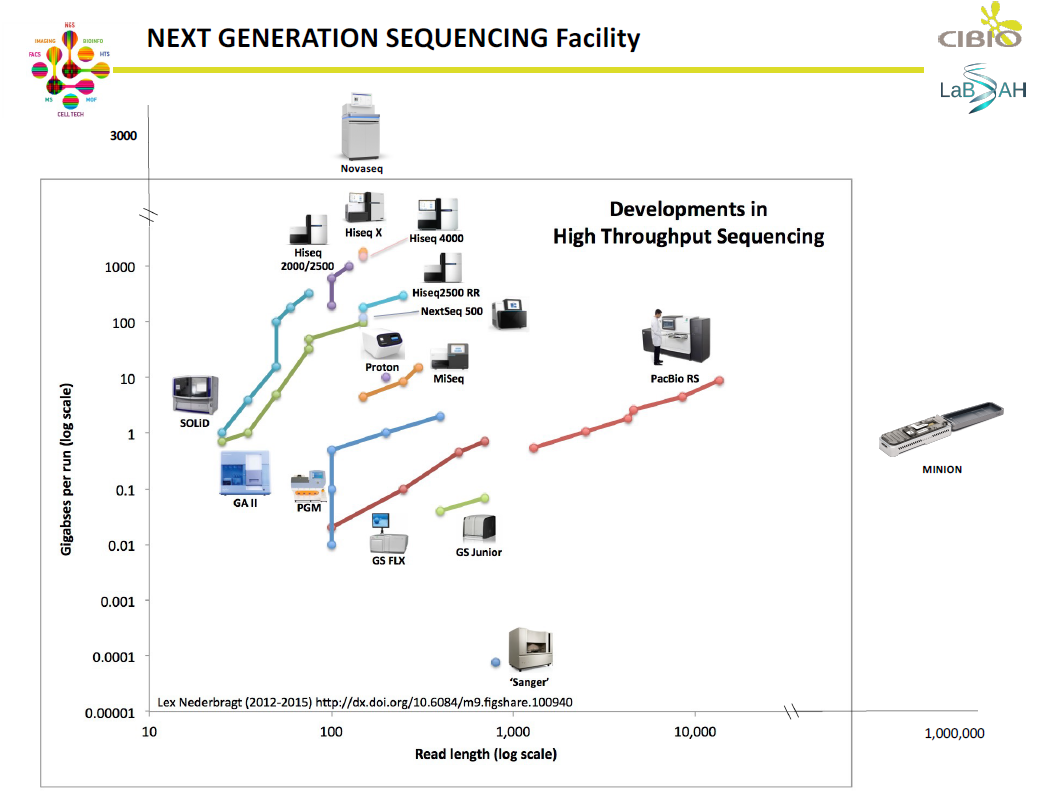
\includegraphics[width=8cm]{sequencingMachines}
\end{figure}




A pletora of sequence machines are available today. None of the machines si able to sequence dna from a sample of blood. 

\subsection{Library preparation}
most of the sequences sequenced are fragmented in short read sequences. effort was spent to generate informations from these sequences.  most of hte times I need polimerization, and primers. we need to add adapters. 

ILLUMINA SEQUENCING:
a good fragment has an unknown sequencei nsiede and two sequences known in the extremes. sequences known to add primers specific. barcodes are something to add to distinguish different samples. clonal amplification is needed to replicate fragments attaached to the solid surface, since machines are not sensible to single molecules


third generation of sequencing: able to read a molecule without replicating it.

at the top of the market there are ILLUMINA machines, that use sequencing by synthesis method. NovaSeq is the biggest one. all the machines use the chemistry base on light emissions. they use reversible terminators, with 3' blocked, use of fluorescence. cleavage of site is made to eliminate the fluorescent signal from a precise nucleotide.  it is then cleaved the block

ILLUMINA uses slide of glass where the sequencing happens, the cell is named flow cell, in the channels there is capability for the fragments to flow. The temperature can ve changed to have different chemical reactions of ligation and separation. The surface is functionalized with a series of primers
Two kids of flow cells, the patterned flow cell permits to create clusters in specific positions, inside nanowalls. all of the fragments can recognize only p5 or p7. once the fragments are attached to the surface, using temperature and solvents flows you can control the sequencing process. attaching the primers to the ligand on the surface means to synthetize the complementary sequence of the DNA to be sequences, so the created DNA is eliminated. bridge-amplification happens, and in htis way is also created the original sequence. at the end it is cutted away one of the two types. the 3' ends are blocked, and a primer is added. 

single index reading
\href{https://www.youtube.com/watch?v=womKfikWlxM}{Video about ILLUMINA}

The sequencing error of ILLUMINA is very low.


Dual index reads: in some cases trough bridge amplification it is also sequenced the index. 

\begin{itemize}
    \item fragmentation
    \item add adaptors through ligation
    \item amplification through clustering
\end{itemize}

\subsection{1-Channel}
\subsection{4-Color Base Calling}
Permits to understand which are  thed correct nucleotide comparing the fluorescence of the other bases, it is use statistics, calculations that the machine makes to understand if statistically it was picked the right base. it is a quality control, if ever it is not overcome the threshold. 
chestity



singles read, 
paired end gives structural informations and also sequence informations.

PACIFIC BIOSCIENCE (PacBio): attach the polymerase to the surface, really small, and light is not able to get out of the wall. it is possible to focus on a particular spot, and for



NANOPORE: proteins modified to have inside, intramembran proteins

